\documentclass[a4paper]{article}
\usepackage[margin=2cm]{geometry}
\usepackage[usenames,dvipsnames]{color}  %% Allow color names
\usepackage{fancyhdr}
\pagestyle{fancy}
\fancyhead[CO,CE]{
                  Programming in C/C++ \\
                  Tjalling Otter \& Emiel Krol
                 }

\usepackage{etoolbox}
\usepackage{placeins}
\usepackage{float}
\usepackage{graphicx}



\setlength\parindent{0pt}

% New page for every section
\let\stdsection\section
\renewcommand\section{\newpage\stdsection}

% New page for every subsection
%\let\stdsubsection\subsection
%\renewcommand\subsection{\newpage\stdsubsection}

% Use for source files
\usepackage{listings}
\lstdefinestyle{cc}{
  title=\lstname,
  belowcaptionskip=1\baselineskip,
  language=C++,
  breaklines=true, %% Wrap long lines
  basicstyle=\small\ttfamily,
  commentstyle=\color{Gray},
  stringstyle=\color{Black},
  keywordstyle=\bfseries\color{OliveGreen},
  identifierstyle=\color{blue},
  numbers=left,
  showstringspaces=false
}

% Use for inline code display in tex
\usepackage{listings}
\lstdefinestyle{in}{
  title=\lstname,
  belowcaptionskip=1\baselineskip,
  language=C++,
  breaklines=true, %% Wrap long lines
  basicstyle=\small\ttfamily,
  commentstyle=\color{Gray},
  stringstyle=\color{Black},
  keywordstyle=\bfseries\color{OliveGreen},
  identifierstyle=\color{blue},
  numbers=left,
  showstringspaces=false,
  aboveskip=-0.5cm
}

% Use for inline display of output/code without highlighting

\lstdefinestyle{text}{
  title=\lstname,
  belowcaptionskip=1\baselineskip,
  breaklines=true, %% Wrap long lines
  basicstyle=\small\ttfamily,
  showstringspaces=false,
  breakautoindent=true,
  numbers=left,
  showlines=true
}

%\newtoggle{aftersection}
%\preto{\lstinputlisting}{\filbreak\global\toggletrue{aftersection}}
%\preto{\subsection}{\iftoggle{aftersection}{\global\togglefalse{aftersection}}{\filbreak}}
%\newcommand{\clearpageafterfirst}{%
%  \gdef\clearpageafterfirst{\clearpage}%
%}

\usepackage{tikz}
\usepackage{tikz-qtree} % For hierarchy

\begin{document}

\section*{Week 4}

\subsection*{Exercise 28}
Note that all of the operator functions are not implemented here, as the point of this code is to show virtual inheritance.

\lstinputlisting[style=cc]{../28/handler/handler.h}
\lstinputlisting[style=cc]{../28/msg/msg.h}
\lstinputlisting[style=cc]{../28/msg/msg.ih}
\lstinputlisting[style=cc]{../28/msg/show.cc}
\lstinputlisting[style=cc]{../28/msg/valueof.cc}
\lstinputlisting[style=cc]{../28/processor/processor.h}

\newpage
\subsection*{Exercise 30}
\begin{itemize}
  \item Draw \texttt{Multi}'s class hierarchy
\end{itemize}
Below is the class hierarchy of \texttt{Multi} at this point of the assignment. \\

\tikzstyle{every node}=[draw=black,thick]
\tikzset{sibling distance=18pt}
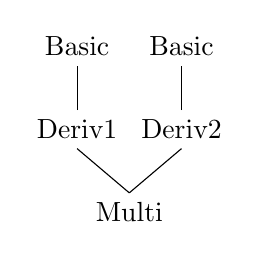
\begin{tikzpicture}[grow=up]
\Tree [.Multi [.Deriv2 Basic ] [.Deriv1 Basic ] ]
\end{tikzpicture}

\begin{itemize}
  \item Explain the compiler's error message after the addition of the \texttt{static\_cast}
\end{itemize}

As can be seen from the illustration above, due to the way that \texttt{Deriv1} and \texttt{Deriv2} are constructed, \texttt{Basic} is included twice by the time \texttt{Multi} inherits from \texttt{Deriv1} and \texttt{Deriv2}. Hence, the compiler indicates that it does not know which \texttt{Basic} to cast to.

\begin{itemize}
  \item Change the statement so that there is no compilation error
\end{itemize}
First, the cast can be done in a two-step fashion: first to either \texttt{Deriv1} or \texttt{Deriv2}, and then to its associated \texttt{Basic}. By doing so, the compiler knows which \texttt{Basic} parent is applicable. This is achieved as follows: \\~\\

\begin{lstlisting}[style=in, caption=c\_multi.cc]
Multi::Multi()
{
  cout << static_cast<Basic *>(static_cast<Deriv1 *>(this)) << '\n';
}
\end{lstlisting}

Secondly, a \texttt{reinterpret\_cast} can be used instead, as follows. What this does is blindly interprets the \texttt{Multi} pointer (\texttt{this}) as a \texttt{Basic} pointer. Note that this is a very dangerous practice, and should be used with extreme caution, as there are a myriad of problems that can arise from this. \\~\\

\begin{lstlisting}[style=in, caption=c\_multi.cc]
Multi::Multi()
{
  cout << reinterpret_cast<Basic *>(this) << '\n';
}
\end{lstlisting}

\begin{itemize}
  \item Show the required modifications to allow the compiler to compile the statement without errors
\end{itemize}

The best way to solve the compilation error without altering the statement would be to make use of virtual inheritance. As such, the class interface of \texttt{Deriv1} and \texttt{Deriv2} should be changed as follows: \\~\\

\begin{lstlisting}[style=in, caption=deriv1.h]
...
class Deriv1: public virtual Basic
{
};
...
\end{lstlisting}
\begin{lstlisting}[style=in, caption=deriv2.h]
...
class Deriv2: public virtual Basic
{
};
...
\end{lstlisting}

\begin{itemize}
  \item How do you realize that this 2nd constructor is the only Basic constructor that's called
\end{itemize}
Without specifying otherwise, \texttt{Multi} directly calls the default constructor of \texttt{Basic}. To change this behaviour, explicitly calling the integer constructor in the initialisation list of \texttt{Multi}, as shown below, is the correct approach. Of course the actual integer used here is just an example. \\~\\
\begin{lstlisting}[style=in, caption=c\_multi.cc]
#include "multi.ih"

Multi::Multi()
:
  Basic(10)
{
  cout << static_cast<Basic *>(this) << '\n';
}
\end{lstlisting}


\newpage
\subsection*{Exercise 32}
\lstinputlisting[style=cc]{../32/fork/fork.h}
\lstinputlisting[style=cc]{../32/fork/fork.ih}
\lstinputlisting[style=cc]{../32/fork/fork.cc}
\lstinputlisting[style=cc]{../32/fork/waitForChild.cc}

\newpage

\end{document}
